\documentclass[letterpaper, 10 pt, conference]{ieeeconf}
%\documentclass[a4paper, 10pt, conference]{ieeeconf}

\IEEEoverridecommandlockouts                      

\overrideIEEEmargins 

%In case you encounter the following error:
%Error 1010 The PDF file may be corrupt (unable to open PDF file) OR
%Error 1000 An error occurred while parsing a contents stream. Unable to analyze the PDF file.
%This is a known problem with pdfLaTeX conversion filter. The file cannot be opened with Acrobat Reader
%Please use one of the alternatives below to circumvent this error by uncommenting one or the other
%\pdfobjcompresslevel=0
%\pdfminorversion=4

% See the \addtolength command later in the file to balance the column lengths
% on the last page of the document

% The following packages can be found on http:\\www.ctan.org
\usepackage{cite}
\usepackage{amsmath,amssymb,amsfonts}
\usepackage{algorithm}
\usepackage{algorithmic}
\usepackage{graphicx}
\usepackage{textcomp}
\usepackage{xcolor}
\usepackage{mathtools}
\usepackage{hyperref}
\def\BibTeX{{\rm B\kern-.05em{\sc i\kern-.025em b}\kern-.08em
    T\kern-.1667em\lower.7ex\hbox{E}\kern-.125emX}}
% \algnewcommand{\StepComment}[1]{\Statex \(\triangleright\)~#1}

\title{\LARGE \bf Multi-Agent Distributed Online Optimization for Floating Offshore Wind Farm Control with Multi-Fidelity Gradient Estimator$^{*}$}

\author{Zekai Chen$^{1}$, Cyrus Neary$^{2}$, and Ryozo Nagamune$^{1}$% <-this % stops a space
\thanks{*This work was supported by the Natural Sciences and Engineering
Research Council of Canada (NSERC) and University of British Columbia Four Year Doctoral Fellowship (4YF).}% <-this % stops a space
\thanks{$^{1}$Zekai Chen and Ryozo Nagamune are with the Department of Mechanical Engineering, the University of British Columbia, Vancouver, BC V6T 1Z4, Canada {\tt\small zkaichen@student.ubc.ca, nagamune@mech.ubc.ca}}%
\thanks{$^{2}$Cyrus Neary is with the Department of Electrical and Computer Engineering, the University of British Columbia, Vancouver, BC V6T 1Z4, Canada {\tt\small cyrus.neary@ubc.ca}}}%


\begin{document}

\maketitle
\thispagestyle{empty}
\pagestyle{empty}

%%%%%%%%%%%%%%%%%%%%%%%%%%%%%%%%%%%%%%%%%%%%%%%%%%%%%%%%%%%%%%%%%%%%%%%%%%%%%%%%
\begin{abstract}
This is the abstract.
\end{abstract}

% \textbf{Keywords:}
% Wind Farm Control

%%%%%%%%%%%%%%%%%%%%%%%%%%%%%%%%%%%%%%%%%%%%%%%%%%%%%%%%%%%%%%%%%%%%%%%%%%%%%%%%
\section{Introduction} \label{sec:introduction}
Introduce the background knowledge, motivation for proposing the framework that uses multi-fidelity methods, conduct a literature review of current work, state the contribution of the paper, and state the organization of the paper. 
\section{Wind Farm Control Problem} \label{sec:problem}
In this section, we first list the assumptions and definitions. Then, we formulate the problem.

\subsection{Assumptions and Definitions} \label{sec:definition}
Consider a wind farm with $N$ floating offshore wind turbines (FOWTs), where $[N]:=\{1,2,\dots,N\}$ denotes the index set. Assume that each FOWT is equipped with sensors that provide measurements of yaw angle ($\gamma$), platform surge ($dx$) and sway ($dy$) motions, power output ($P$), and wind conditions ($v$). Let $k$ denote the discrete time step.

Following previous work on turbine repositioning, the control input of each FOWT$_n$ is the nacelle yaw angle at time step $k$, denoted by $\gamma_{n,k}$. To enable distributed control, we define the neighbor set $\mathcal{N}_n$ of FOWT$_n$ as the set of turbines whose wakes aerodynamically influence FOWT$_n$. Thus, the specific members of $\mathcal{N}_n$ depend on the wind farm layout and the indexing of the turbines. For simplicity, we denote the neighboring turbines by $\{\text{FOWT}_m\}_{m \in \mathcal{N}_n}$.

The objective of wind farm control is to improve farm-level performance by mitigating wake effects. For turbine repositioning, moving turbines out of the wake not only increases power capture but also tends to reduce structural loading, since the wake is a source of both power loss and increased loads. Therefore, the goal of mitigating wake effects is closely coupled to increasing power capture, and the cost function is defined accordingly. Let $P_n^{\text{rate}}$ denote the rated power output of FOWT$_n$, and let $P_{n,k}^{\text{real}}$ denote its actual power output at time step $k$. The local cost of FOWT$_n$ is defined as
\begin{equation} \label{eq:cost_def}
    f_{n,k} = - \frac{P_{n,k}^{\text{real}}}{P_n^{\text{rate}}} .
\end{equation}

Since FOWT$_n$ and its neighbors $\{\text{FOWT}_m\}_{m \in \mathcal{N}_n}$ are aerodynamically coupled, $f_{n,k}$ depends on both $\gamma_{n,k}$ and the yaw angles of its neighbors. Accordingly, the local cost of FOWT$_n$ can be written as $f_{n,k}\!\left(\gamma_{n,k}, \{\gamma_{m,k}\}_{m \in \mathcal{N}_n}\right)$. The farm-level cost is then defined as the sum of the local costs:
\begin{equation} \label{eq:cost_sum}
    f_k(\Gamma_k) = \sum_{n=1}^N f_{n,k}\!\left(\gamma_{n,k}, \{\gamma_{m,k}\}_{m \in \mathcal{N}_n}\right),
\end{equation}
where $\Gamma_k = (\gamma_{1,k}, \gamma_{2,k}, \dots, \gamma_{N,k})$ denotes the vector of yaw angles of all turbines at time step $k$. According to \eqref{eq:cost_def}, $f_{n,k}$ decreases as the power output of FOWT$_n$ increases. Therefore, minimizing $f_k(\Gamma_k)$ is equivalent to maximizing the total normalized power output of the wind farm, thereby improving farm-level performance.

\subsection{Problem Formulation}
Based on the above definition, we formulate the problem under a multi-agent coordination-based distributed online optimization framework: at each time step $k \geq 1$, FOWT$_n$ makes a control action $\gamma_{n,k}$ based on information of its own and $\{\text{FOWT}_m\}_{m \in \mathcal{N}_n}$, which includes $f_{n,\ell}, \gamma_{m,\ell}, \gamma_{n,\ell}$ with $\ell\leq k-1$. Subsequently, the environment reveals $f_{n,k}\!\left(\gamma_{n,k},\,\{\gamma_{m,k}\}_{m\in\mathcal{N}_n}\right)$. Each turbine then shares its information with its neighbor, and the process repeats at every time step until a pre-specified horizon $T>0$ is reached.

Assume the maximum yaw angle is denoted by $\gamma_{\max}$ and let $X_n=\{\gamma : |\gamma| \le \gamma_{\max}\}$ denote the feasible set of FOWT$_n$. Therefore, the corresponding objective of the problem is to minimize the following cumulative cost:
\begin{equation} \label{eq:opti2}
\begin{aligned}
    \min_{\substack{\gamma_{n,k} \\ n\in[N]}} \quad
    & \sum_{k=1}^{T}\sum_{n=1}^{N} f_{n,k}\!\left(\gamma_{n,k},\,\{\gamma_{m,k}\}_{m\in\mathcal{N}_n}\right) \\
    \text{s.t.}\quad
    & \gamma_{n,k} \in X_n, \quad \forall n\in[N],\; \forall k.
\end{aligned}
\end{equation}
\section{Methodology} \label{sec:method}
Based on the above definitions and formulation, we designed the methodology.
\subsection{Gradient Estimation} \label{sec:gradest}
As previously analyzed, one big obstacle is that no analytic gradient of $f_{n,k}$ is available. Hence, gradients must be estimated from sampling data alone. We adopt the one-point bandit estimator for its simplicity, and the two-point bandit estimator for its lower variance, and briefly contrast it with the central-difference estimator.

\emph{One-point estimator.} Querying the current point,
\begin{equation} \label{eq:one-bandit}
\begin{aligned}
    \hat{g}_{n,k} := \frac{d_n}{\delta_k}
    &\Big( f_{n,k}\!\left(\gamma_{n,k} + \delta_k u_{n,k},\,\{\gamma_{m,k}\}_{m\in\mathcal{N}_n}\right) \Big)u_{n,k},
\end{aligned}
\end{equation}
where $u_{n,k} \sim \mathbb{S}^{d_n-1}$ is uniform and $\delta_k > 0$ is an exploration parameter. Since each yaw $\gamma_{n,k}$ is scalar, $d_n = 1$ and $u_{n,k} \in \{-1,+1\}$.

\emph{Two-point estimator.} Moreover, we can also adopt a two-point bandit estimator, which normally yields better performance compared to the one-point bandit estimator~\cite{li2023survey}. Querying the current point and one perturbed point,
\begin{equation} \label{eq:two-bandit}
\begin{aligned}
    \hat{g}_{n,k} := \frac{d_n}{\delta_k}
    &\Big( f_{n,k}\!\left(\gamma_{n,k} + \delta_k u_{n,k},\,\{\gamma_{m,k}\}_{m\in\mathcal{N}_n}\right) \\
    &\quad - f_{n,k}\!\left(\gamma_{n,k},\,\{\gamma_{m,k}\}_{m\in\mathcal{N}_n}\right)\Big)
    u_{n,k}.
\end{aligned}
\end{equation}

\emph{Central-difference estimator.} An alternative way to estimate the gradient, with the same bias but lower variance, is by adopting the central-difference formula, defined as:
\begin{equation} \label{eq:cen-diff}
\begin{aligned}
    \hat{g}_{n,k} = \frac{1}{2\delta_k}\Big(
        & f_{n,k}\!\left(\gamma_{n,k} + \delta_k,\,\{\gamma_{m,k}\}_{m\in\mathcal{N}_n}\right) \\
        & - f_{n,k}\!\left(\gamma_{n,k} - \delta_k,\,\{\gamma_{m,k}\}_{m\in\mathcal{N}_n}\right)\Big)
\end{aligned}
\end{equation}

Both two points estimators are unbiased for the gradient of the smoothed function $\hat{f}_{n,k,\delta}(\cdot) = \mathbb{E}_{w \sim B^{d_n}}[f_{n,k}(\cdot + \delta w)]$, where $B^{d_n}$ denotes the unit ball in $\mathbb{R}^{d_n}$; i.e., $\mathbb{E}[\hat{g}_{n,k}] = \nabla_{\gamma_n} \hat{f}_{n,k,\delta}$, and $\hat{f}_{n,k,\delta} \to f_{n,k}$ as $\delta_k \to 0$. The two-point estimator subtracts the zero-mean term $f_{n,k}(\gamma_{n,k}) u_{n,k}$, which acts as a control variate, while the central-difference estimator removes the probe-direction randomness altogether, so both reduce variance without introducing bias. However, the central-difference estimator requires one extra probe per turbine, raising the number of points required for computation per step from $N+1$ to $2N+1$. Moreover, to ensure the probe remains feasible, the probe is performed on a shrunk set (e.g., $(1-\xi_k)X_n$, $\xi_k \in (0,1)$)~\cite{yi2022regret}.

\section{Algorithm} \label{sec:algorithm}
In this section, we design the distributed online algorithm with bandit feedback gradient estimation. Based on Equation~\ref{eq:cost_sum}, the partial derivative of the $f_k$ with respect to $\gamma_{n,k}$ can be decomposed as
\begin{equation}
    \frac{\partial f_k}{\partial \gamma_{n,k}}
    = \frac{\partial f_{n,k}}{\partial \gamma_{n,k}}
    + \sum_{m \in \mathcal{N}_n} \frac{\partial f_{m,k}}{\partial \gamma_{n,k}},
    \label{eq:coord}
\end{equation}
where $\sum_{m \in \mathcal{N}_n} \partial f_{m,k}/\partial \gamma_{n,k}$ represents the aggregate sensitivity of the neighboring turbines’ costs to the yaw action of FOWT$_n$, i.e., the wake-induced coupling. Each term in Equation~\ref{eq:coord} is estimated by the gradient estimator in Section~\ref{sec:gradest}: FOWT$_n$ estimates $\partial f_{n,k}/\partial \gamma_{N,K}$ by probing its own yaw, while $\{\text{FOWT}_m\}_{m \in \mathcal{N}_n}$ estimates $\partial f_{m,k}/\partial \gamma_{n,k}$ by probing FOWT$_n$. 

As introduced, gradient estimation requires perturbing the physical systems randomly, which is impractical for real FOWFs. Therefore, to ensure practical feasibility, we design two algorithms based on the auxiliary tools that are used to acquire the gradient information: a low-fidelity method and a multi-fidelity method in the following chapter.

\subsection{Low-Fidelity Method}
In this method, we use a quasi-static low-fidelity simulator, the Floating Offshore Wind Farm Simulator (FOWFSim)~\cite{FOWFSim} (based on FLORIS and MoorPy), to probe the system to approximate the gradient, as Figure~\ref{fig:LF_BD} shows. It is important to note that this framework should be able to work when replacing the high-fidelity and low-fidelity models. The overall workflow is as follows. At each time step $k$, the high-fidelity dynamic simulator passes the relevant state information to the quasi-static low-fidelity simulator. Then, the gradient vector $\hat{G}_k$ is estimated, after which the vector that records optimal yaw angles $\Gamma_{k+1}$ is derived and returned to the high--fidelity simulator. The dynamic simulator updates the turbine states accordingly, and the process repeats. 

\begin{figure}[h]
    \centering
    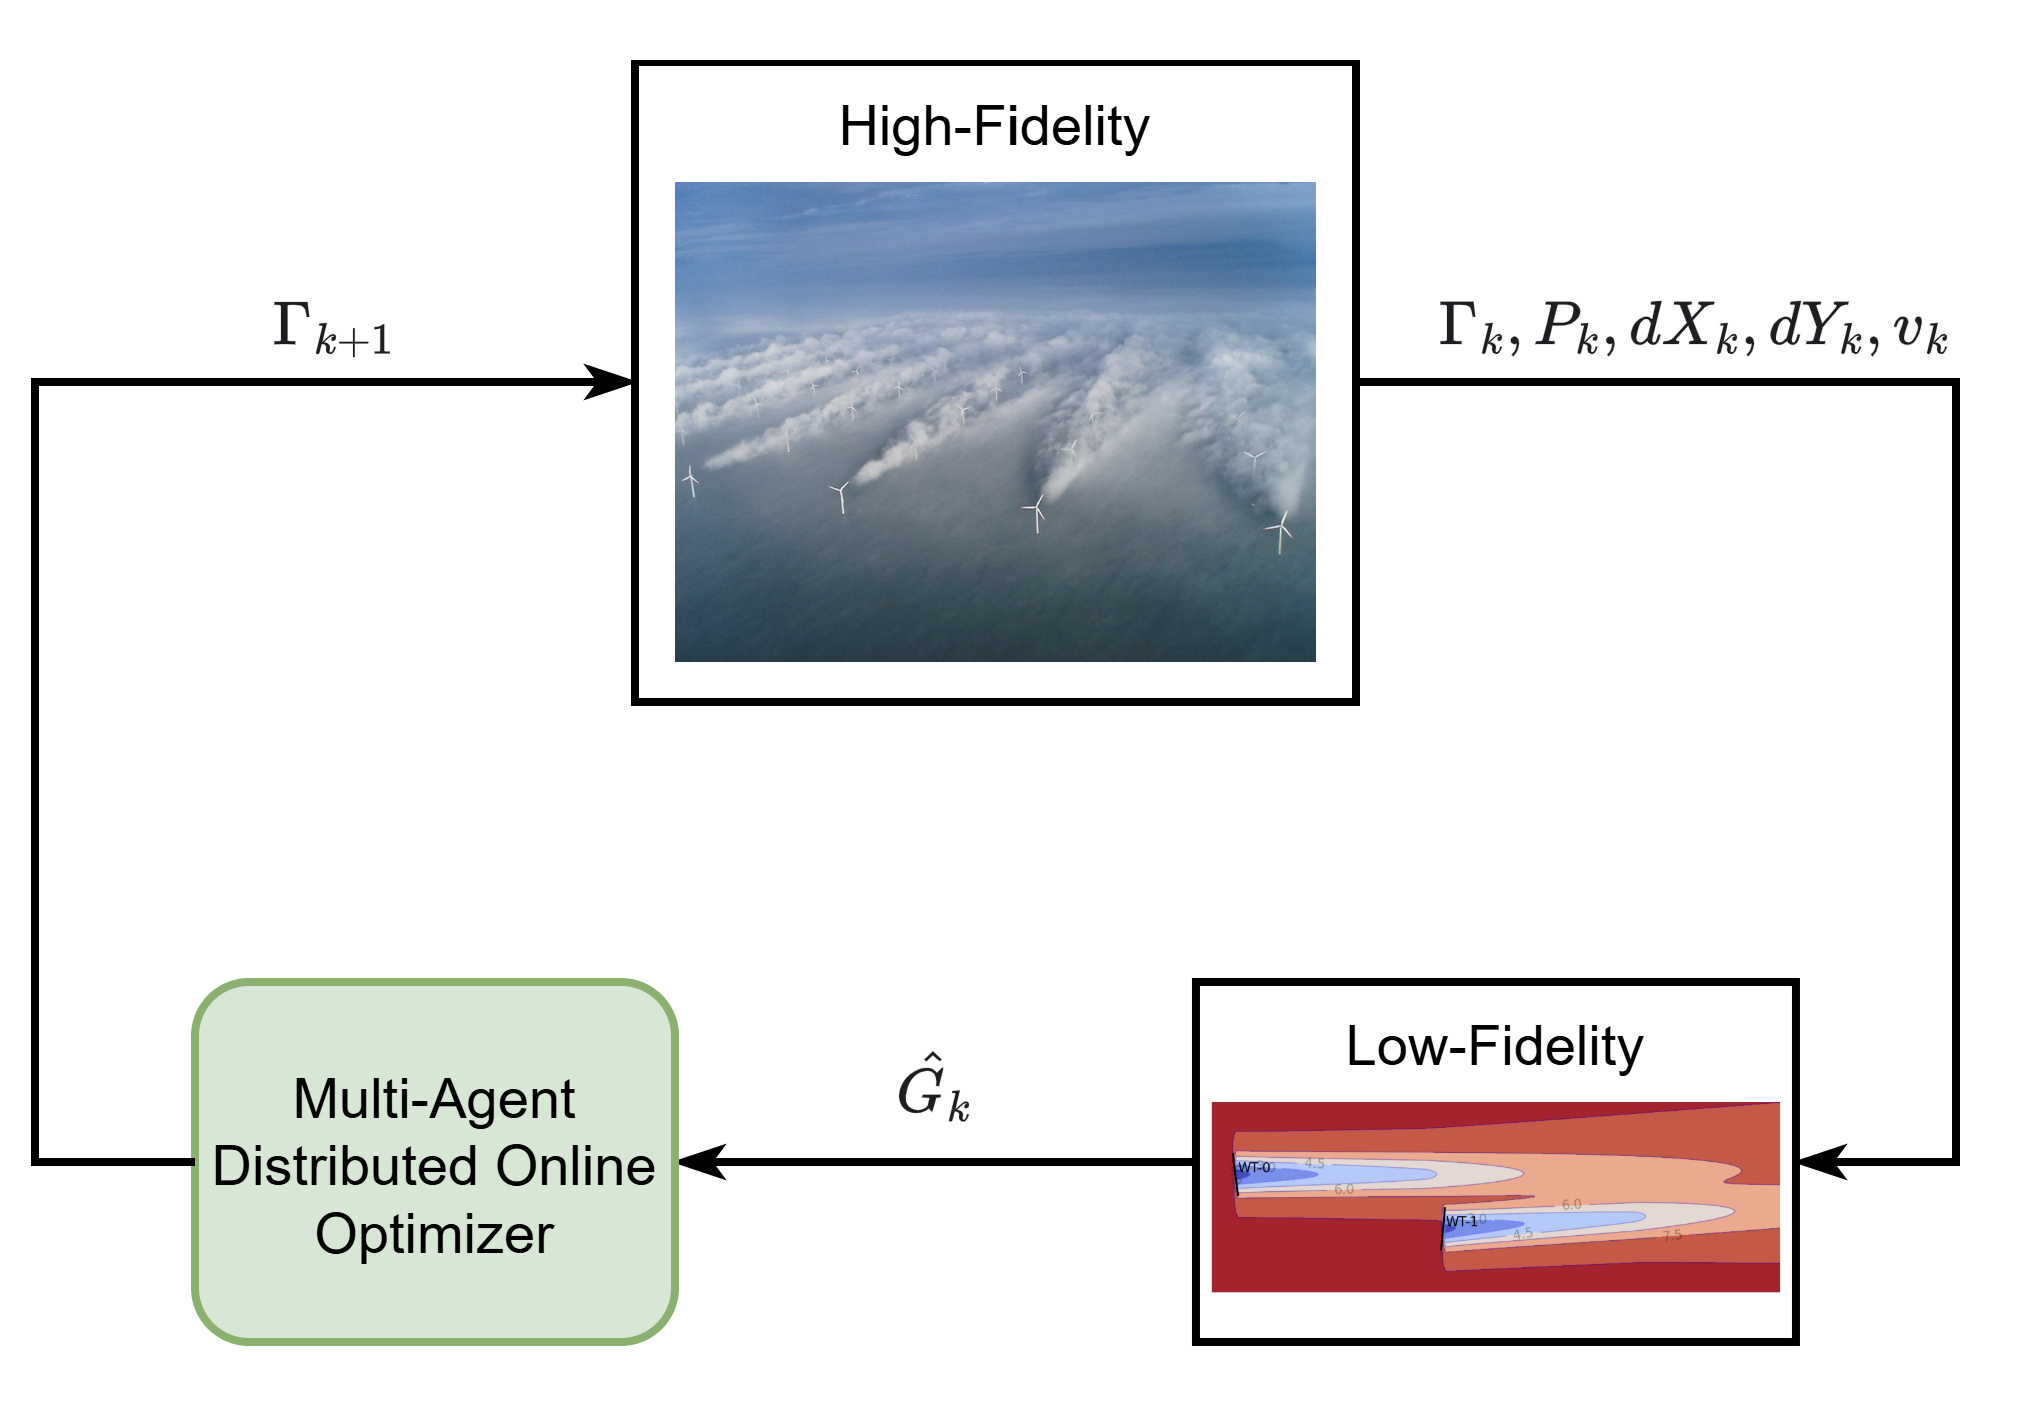
\includegraphics[width=\linewidth]{overleaf/figures/LF_BD.png}
    \caption{Structure of the proposed low-fidelity method at each time step $k$. Uppercase letters denote vectors.}
    \label{fig:LF_BD}
\end{figure}

The proposed method is summarized in Algorithm~\ref{alg:doo}, in which $\mathcal{P}_{X_n}$ denotes the Euclidean projection onto $X_n$.
\begin{algorithm}[h!]
\caption{Low-Fidelity Method.}
\label{alg:doo}
\begin{algorithmic}
    \STATE \textbf{Input:} stepsize $\{\alpha_k\}$; exploration $\{\delta_k\}$; shrinkage $\{\xi_k\} \subset (0,1)$ with $\delta_k \le r(X_n)\xi_k$.
    \STATE \textbf{Initialize:} $\gamma_{n,1} \in (1-\xi_1)X_n$ for all $n \in [N]$ (one sign quadrant fixed).
    \FOR{$k = 1, 2, \dots$}
        \FOR{$n = 1, \dots, N$ (sequentially)}
            \STATE Draw $u_{n,k} \in \{-1,+1\}$ uniformly at random; evaluate $f_{\kappa,k}$ at $\gamma_{n,k}$ and $\gamma_{n,k}+\delta_k u_{n,k}$ for all $\kappa\in\{n\}\cup\mathcal{N}_n$, keeping every other yaw fixed at its committed value;
        \ENDFOR
        \FOR{$n = 1, \dots, N$ in parallel}
            \STATE Own partial estimate:
            \begin{equation}
                \hat{g}_{n,k}^{(n)} = \frac{u_{n,k}}{\delta_k}\Big(f_{n,k}(\gamma_{n,k}+\delta_k u_{n,k},\cdot) - f_{n,k}(\gamma_{n,k},\cdot)\Big);
            \end{equation}
            \STATE Receive cross-partial estimates from each $m \in \mathcal{N}_n$:
            \begin{equation}
                \hat{g}_{m,k}^{(n)} = \frac{u_{n,k}}{\delta_k}\big(f_{m,k}(\gamma_{n,k}+\delta_k u_{n,k},\cdot)-f_{m,k}(\gamma_{n,k},\cdot)\big);
            \end{equation}
            \STATE Assemble:
            \begin{equation}
                \hat{g}_{n,k} = \hat{g}_{n,k}^{(n)} + \sum_{m \in \mathcal{N}_n}\hat{g}_{m,k}^{(n)};   
            \end{equation}
            \STATE Update:
            \begin{equation}
                \gamma_{n,k+1} = \mathcal{P}_{(1-\xi_{k+1})X_n}\big(\gamma_{n,k} - \alpha_{k}\hat{g}_{n,k}\big);
            \end{equation}
        \ENDFOR
    \ENDFOR
    \STATE \textbf{Output:} $\{\gamma_{n,k}\}$.
\end{algorithmic}
\end{algorithm}

\subsection{Multi-Fidelity Method}
The previous method purely relies on a low-fidelity simulator that is built on simplifying assumptions about the external environmental conditions and only captures the steady-state wake dynamics. However, the real wind farm is dynamic, and a controller optimized purely on such a low-fidelity model cannot bridge the sim-to-real gap. To retain the sample efficiency of the low-fidelity simulator while anchoring the estimate to the true dynamics, we adopt a multi-fidelity framework~\cite{peherstorfer2018survey}. Specifically, we implement the fusion via the control variate method. 

Let $\hat{g}^{h}_{n,k}$ and $\hat{g}^{l}_{n,k}$ denote the gradient estimates of FOWT$_n$ obtained from the high-fidelity (dynamic) simulator and the low-fidelity (quasi-static) simulator, respectively, using the gradient estimator in Section~\ref{sec:gradest}. The two estimates are made correlated by probing both simulators with the same perturbation direction $u_{n,k}$ and by initializing the low-fidelity simulator at the current high-fidelity state.

The key difficulty in a dynamic, non-stationary environment is that the high-fidelity probes are spread across consecutive time steps: the base measurement is taken at instant $\tau_0$ under inflow $w_0$, while the probe of FOWT$_n$ is taken at a later instant $\tau_i$ under inflow $w_i$. A naive high-fidelity difference therefore mixes the yaw effect with the environmental drift $w_i - w_0$. To remove this drift, we probe both fidelities \emph{jointly}: at every high-fidelity query instant we also evaluate the low-fidelity model at the \emph{same} time, wind, and yaw, using the \emph{same} perturbation direction $u_{n,k}$. For the own partial of FOWT$_n$ this yields three estimates:
\begin{equation} \label{eq:mf-drifted}
\begin{aligned}
\hat{g}^{h}_{n,k} &= \frac{u_{n,k}}{\delta_k}\big(f^{h}(\gamma_{n,k}+\delta_k u_{n,k},\,w_i) - f^{h}(\gamma_{n,k},\,w_0)\big),\\
\hat{g}^{l}_{n,k} &= \frac{u_{n,k}}{\delta_k}\big(f^{l}(\gamma_{n,k}+\delta_k u_{n,k},\,w_i) - f^{l}(\gamma_{n,k},\,w_0)\big),\\
\hat{g}^{l,\mathrm{cln}}_{n,k} &= \frac{u_{n,k}}{\delta_k}\big(f^{l}(\gamma_{n,k}+\delta_k u_{n,k},\,w_0) - f^{l}(\gamma_{n,k},\,w_0)\big),
\end{aligned}
\end{equation}
where $\hat{g}^{l,\mathrm{cln}}_{n,k}$ is the clean, synchronous low-fidelity gradient (both probes evaluated under $w_0$, while $\hat{g}^{l}_{n,k}$ is the \emph{drifted} low-fidelity gradient computed over the same two instants as $\hat{g}^{h}_{n,k}$. The fused estimate takes the low-fidelity gradient as the anchor and the high-minus-low difference as a correction:
\begin{equation} \label{eq:mf-gradient}
    \hat{g}_{n,k} = \hat{g}^{l,\mathrm{cln}}_{n,k} + c_{n,k}\big(\hat{g}^{h}_{n,k} - \hat{g}^{l}_{n,k}\big).
\end{equation}
Because the environmental drift contaminates $\hat{g}^{h}_{n,k}$ and $\hat{g}^{l}_{n,k}$ alike, it cancels in the difference, so the correction retains only the high-fidelity yaw effect. With $c_{n,k}\to 1$ the fused estimate is unbiased toward the high-fidelity gradient, while when the correction is small it degrades gracefully to the low-fidelity behavior alone.

Let $A_{n,k} := \hat{g}^{l,\mathrm{cln}}_{n,k}$ denote the anchor and $D_{n,k} := \hat{g}^{h}_{n,k} - \hat{g}^{l}_{n,k}$ the drift-free correction, so that $\hat{g}_{n,k} = A_{n,k} + c_{n,k} D_{n,k}$. The variance of the fused estimate is $\mathrm{Var}(A_{n,k}) + c_{n,k}^2 \mathrm{Var}(D_{n,k}) + 2 c_{n,k}\mathrm{Cov}(A_{n,k}, D_{n,k})$, which is minimized by
\begin{equation} \label{eq:mf-cv}
    c^{*}_{n,k} = -\frac{\mathrm{Cov}(A_{n,k},\,D_{n,k})}{\mathrm{Var}(D_{n,k})}
    = -\frac{\mathrm{Cov}(\hat{g}^{l,\mathrm{cln}}_{n,k},\,\hat{g}^{h}_{n,k}-\hat{g}^{l}_{n,k})}{\mathrm{Var}(\hat{g}^{h}_{n,k}-\hat{g}^{l}_{n,k})}.
\end{equation}
In practice, $c^{*}_{n,k}$ is estimated online from the stream of anchor--correction pairs $(A_{n,k},\,D_{n,k})$ using sample statistics, maintained across time steps with an exponential moving average of the moments $\mathbb{E}[A D]$, $\mathbb{E}[A]$, $\mathbb{E}[D]$, and $\mathbb{E}[D^2]$~\cite{liu2025multi}. The coefficient is initialized to $c_{n,1}=0$ (low-fidelity only) and clamped to $[0,1]$, so that $c=0$ recovers the low-fidelity estimate and $c=1$ the drift-corrected high-fidelity estimate. The fusion in Equation~\ref{eq:mf-gradient} is applied to each partial gradient term in Equation~\ref{eq:coord} before they are assembled, and the low-fidelity correction is evaluated at the \emph{measurement} time of each high-fidelity probe so that the drift remains common-mode and cancels. 
\begin{itemize}
    \item \textcolor{purple}{Maybe I should try one-point estimation to match the time?}
    \item \textcolor{purple}{How to combine a steady-state map with dynamic data?}
\end{itemize}


\begin{algorithm}
\caption{Multi-Fidelity Method.}
\label{alg:doo-mf}
\begin{algorithmic}
    \STATE \textbf{Input:} stepsize $\{\alpha_k\}$; exploration $\{\delta_k\}$; shrinkage $\{\xi_k\} \subset (0,1)$ with $\delta_k \le r(X_n)\xi_k$.
    \STATE \textbf{Initialize:} $\gamma_{n,1} \in (1-\xi_1)X_n$ for all $n \in [N]$ (one sign quadrant fixed).
    \FOR{$k = 1, 2, \dots$}
        \FOR{$n = 1, \dots, N$ (sequentially)}
            \STATE Draw $u_{n,k} \in \{-1,+1\}$ uniformly at random; evaluate $f_{\kappa,k}$ at $\gamma_{n,k}$ and $\gamma_{n,k}+\delta_k u_{n,k}$ for all $\kappa\in\{n\}\cup\mathcal{N}_n$, keeping every other yaw fixed at its committed value;
        \ENDFOR
        \FOR{$n = 1, \dots, N$ in parallel}
            \STATE At each high-fidelity query instant, evaluate the low-fidelity model at the same time.
            \STATE Own partial estimate via the fused gradient in Eq.~\eqref{eq:mf-gradient}:
            \begin{equation}
                \hat{g}_{n,k}^{(n)} = \hat{g}^{l,\mathrm{cln}(n)}_{n,k} + c_{n,k}\big(\hat{g}^{h(n)}_{n,k} - \hat{g}^{l(n)}_{n,k}\big);
            \end{equation}
            \STATE Receive cross-partial estimates from each $m \in \mathcal{N}_n$, fused analogously:
            \begin{equation}
                \hat{g}_{m,k}^{(n)} = \hat{g}^{l,\mathrm{cln}(n)}_{m,k} + c_{n,k}\big(\hat{g}^{h(n)}_{m,k} - \hat{g}^{l(n)}_{m,k}\big);
            \end{equation}
            \STATE Assemble:
            \begin{equation}
                \hat{g}_{n,k} = \hat{g}_{n,k}^{(n)} + \sum_{m \in \mathcal{N}_n}\hat{g}_{m,k}^{(n)};   
            \end{equation}
            \STATE Update:
            \begin{equation}
                \gamma_{n,k+1} = \mathcal{P}_{(1-\xi_{k+1})X_n}\big(\gamma_{n,k} - \alpha_{k}\hat{g}_{n,k}\big);
            \end{equation}
        \ENDFOR
    \ENDFOR
    \STATE \textbf{Output:} $\{\gamma_{n,k}\}$.
\end{algorithmic}
\end{algorithm}

%%%%%%%%%%%%%%%%%%%%%%%%%%%%%%%%%%%%%%%%%%%%%%%%%%%%%%%%%%%%%%%%%%%%%%%%%%%%%%%%
\section*{ACKNOWLEDGMENT}
DeepSeek V4 Pro large language model~\cite{deepseek} is used for editing the paper.

%%%%%%%%%%%%%%%%%%%%%%%%%%%%%%%%%%%%%%%%%%%%%%%%%%%%%%%%%%%%%%%%%%%%%%%%%%%%%%%%
\bibliographystyle{IEEEtran}
\bibliography{ref}

\end{document}